\documentclass[12pt, titlepage]{article}

\usepackage{graphicx}
\usepackage{wrapfig}
\usepackage{hyperref}
\usepackage{siunitx}
\usepackage{amsmath}
\usepackage{enumerate}

\title{Flippin' Flingers Trebuchet Final Report}
\author{Omar Ebrahim 110076575\\Saif Kaoud 110076323\\[10pt] Dr. John Magliaro\\
University of Windsor}

\begin{document}
    \maketitle
    \section{Abstract}
    This final report provides an overview of the finalization of the project focused on the sketching, designing, and modeling of a trebuchet.\\[10pt]
    The report outlines the key milestones achieved since the inception of the project, 
    including build process, changes from the initial design, detailed component specifications, analytical-numerical-physical test results, and dicussion on test results.\\[10pt]
    The report utilizes CAD, first principles, numerical simulations, and physical tests to achieve this goal.
    \newpage
    \tableofcontents
    \listoffigures
    \newpage
    \section{Introduction}
    This report's mission statement is to summarize the team's final results with:
    \begin{itemize}
        \item Detailed CAD drawings.
        \item Analytical Calculations.
        \item Numerical modeling.
        \item Real-life data.
    \end{itemize}
    The problem outline is to design and analyze the trebuchet to maximize
    projectile distance and accuracy.\\[10pt]
    The trebuchet is designed for maximum distance through general
    plane motion.\footnote{Hibbeler, 2015}It is also designed for maximum 
    accuracy through string measure.\footnote{Rhoten, 2021}\\[10pt]
    To maximize distance, the velocity of the projectile is considered, as
    distance and velocity are proportional. Increasing the counterweight 
    fall distance can boost the projectile's velocity.\footnote{Siano, 2001}
    Increasing the counterweight-to-launch distance increases the velocity 
    of the projectile.\footnote{Denny, 2005}\\[10pt]
    Lastly, adjusting the trebuchet firing angle to 
    45 degrees achieves the maximum projectile distance.\footnote{Connel, 2001}
    \newpage
    \section{Methodology}
    The team uses CATIA, a CAD software, to design components and present
    them in detailed technical drawings.\\[10pt] 
    Next, the team applies the principles of Kinematics and Kinetics to analyze the motion of the trebuchet. 
    Through this analysis, they are able to make accurate estimations regarding the distance the projectiles will travel.\\[10pt]
    The team also utilizes Working Model 2D, a CAE software, to numerically simulate the trebuchet's motion and provide numerical data for analyzing the impact of various factors on its performance.\\[10pt]
    Finally, the team conducts real-life tests of the trebuchet to compare and contrast the actual results with their analytical and numerical predictions. They carefully analyze the variations between the expected and observed outcomes, discussing the factors that contribute to these differences.    
    \newpage
    \section{Design}
    \subsection{CAD}
    Figure \ref{CAD} showcases the CAD model of the Floating Arm Trebuchet. The design features a robust physical body. The counterweight is attachable to the middle axle, and the arm holds the sling and guide chute at the end. To enhance portability, wheels are attachable to the corners of the base, facilitating easy transportation of the trebuchet.\\
    \begin{figure}[t]                                  
    \centering
    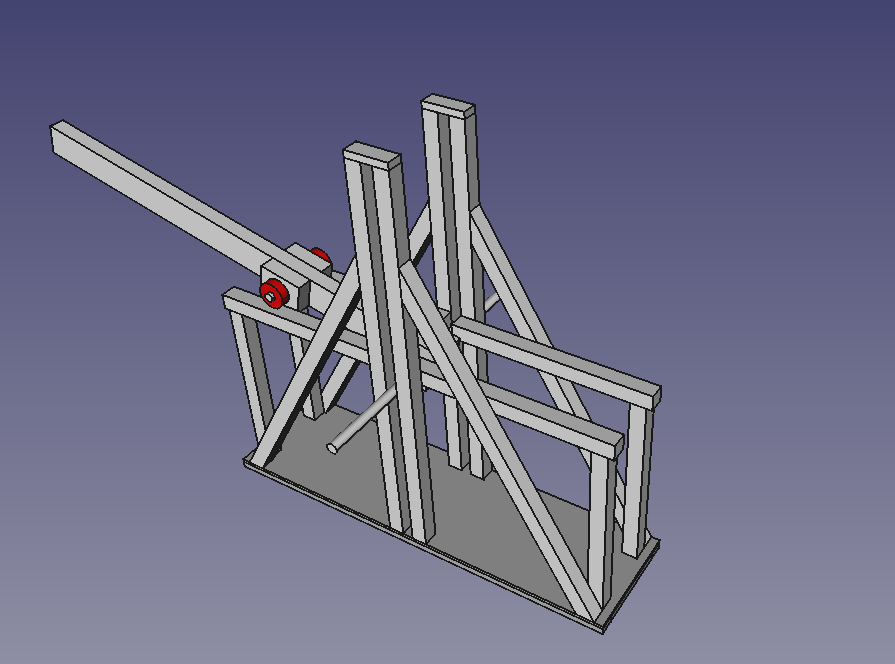
\includegraphics[width=0.8\textwidth]{CAD.png}
    \caption{Floating Arm Trebuchet in CAD\label{CAD}}
    \end{figure}
    \newpage
    \subsection{Technical Drawings}
    \newpage
    \section{Results}
    \subsection{Analytical Calculations}
    \begin{figure}[b]                                  
    \centering
    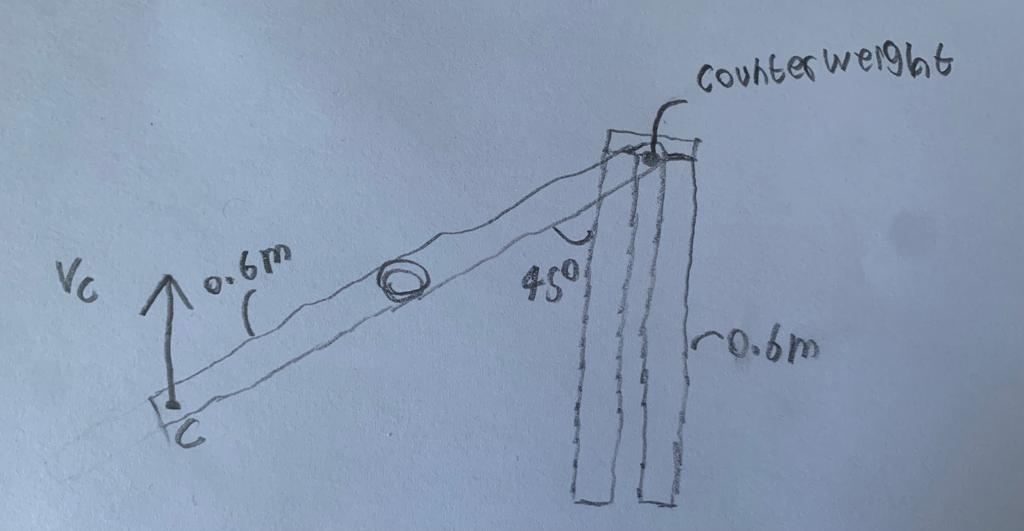
\includegraphics[width=0.45\textwidth]{d1.jpeg}
    \caption{Diagram\label{d1}}
    \end{figure}
    Before the team can begin to analyze the motion of the trebuchet, they must
    first take some measurements. The team measures the length of the arm to be 
    approximately $0.6$ m. The team uses two 355mL drink cans.
    Therefore, the mass of the counterweight is $\frac{2*355}{1000} \approx 0.7$ kg.
    The mass of the arm with the supporting wheels is $0.3$ kg.
    Hence, the combined mass of the counterweight with the arm is 
    $0.7 + 0.3 = 1$ kg. The team measured the radius
    and height of the cans which were $0.066$ m and $0.12$ m respectively. See Figure \ref{d1}.\\[20pt]
    Given: $m_{a} = 0.3$ kg, $m_{w} = 0.7$ kg, $m = 1$ kg, $l = h = 0.6$ m, $\theta = 45^\circ$
    $r = 0.066$ m and $h_c = 0.12$ m\\
    RTF: Range of projectile, $s$\\
    Assumptions: Rigid bodies, no energy loss, starts from rest.\\[10pt]
    To solve this problem, the team uses the General Work-Energy Equation:
    $$T_1 + \Sigma U_{1-2} = T_2$$
    Since, the trebuchet starts from rest, $T_1 = 0$. Now, to find $\Sigma U_{1-2}$,
    $$\Sigma U_{1-2} = mgh = (1)(9.8)(0.6) = 5.88 \approx 5.9 \mathrm{J}$$
    To find $T_2$, the team needs to find the equivalent mass moment of inertia $I_e$,
    $$I_e = I_a + I_w$$
    \newpage
    \noindent The team assumes the arm to be a rod, and the counterweight to be a cylinder. Therefore,
    \begin{align*}
        I_e &= \frac{1}{12}m_al^2 + \frac{1}{12}m_w(3r^2 + h_c^2) \\
        &= \frac{1}{12}(0.3)(0.6)^2 + \frac{1}{12}(0.7)\left(3(0.066)^2 + (0.12)^2\right) = 0.0106 \, \mathrm{kg} \cdot \mathrm{m}^2
    \end{align*}
    To find $T_2$ we need to relate $\omega$ with v, the team uses the kinematic equation for rotational motion,
    $$v = \omega l;\; \omega = \frac{v}{l}$$
    Substituting this into the kinetic energy equation,
    \begin{align*}
        T_2 &= \frac{1}{2}mv^2 + \frac{1}{2}I_e\left(\frac{v}{l}\right)^2 \\
        &= \frac{1}{2}(1)v^2 + \frac{1}{2}(0.0106)\left(\frac{v}{0.6}\right)^2 \\
        &= 0.5v^2 + 0.0147v^2 = 0.5147v^2
    \end{align*}
    Now, substituting $\Sigma U_{1-2}$ and $T_2$ into the General Work-Energy Equation,
    $$5.9 = 0.5147v^2$$
    $$v = v_e = 3.38 \, \mathrm{m/s};\; \omega = \frac{3.38}{0.6} = 5.63 \, \mathrm{rad/s}$$
    Now, to find the velocity of point C, the team uses the kinematic equation for rotational motion assuming the distance from the equivalent center to point C is $0.5$ m,
    $$v_c = v_e + \omega l_{c/e} = 3.38 + (5.63)(0.5) = 6.2 \, \mathrm{m/s}$$
    Now, to find the range of the projectile, the team uses the parabolic motion equation assuming that the time right before the ball lands is 4 seconds,
    $$v_c = \frac{ds}{dt};\; \displaystyle\int_{0}^{s}ds = \displaystyle\int_{0}^{4}6.2dt$$
    \[ \boxed{s = 24.8 \, \mathrm{m}} \]
    From this analysis, the team predicts that the trebuchet will launch the projectile 24.8 meters.
    \newpage
    \subsection{Numerical Model}
    The Floating Arm Trebuchet implemented in Working Model 2D can be found 
    in Figure \ref{model}. Additionally, a tracing of the trebuchet's motion 
    can be found in Figure \ref{motion}. Tracing is a feature in Working 
    Model 2D that shows each frame of the motion of an object.\\[10pt]
    Lastly, position-velocity-acceleration graphs for both vertical and 
    horizontal axes of the projectile are found in Figure \ref{graphs}.
    The horizontal velocity of the ball increases linearly once the trebuchet fires
    then stays constant (ignoring air resistance). Hence, the team predicts 
    with this model that they can achieve around 20 meters of projectile
    distance.

    \begin{figure}[t]                                  
    \centering
    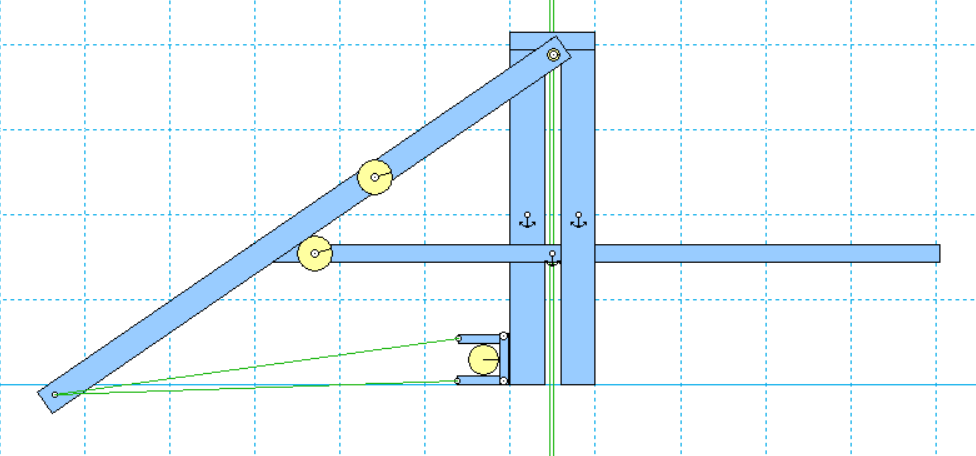
\includegraphics[width=0.7\textwidth]{Model.png}
    \caption{Floating Arm Trebuchet model in Working Model 2D\label{model}}
    \end{figure}

\begin{figure}[b]
    \begin{minipage}[t]{0.69\textwidth}
        \vspace{12pt}
        \begin{flushleft}
            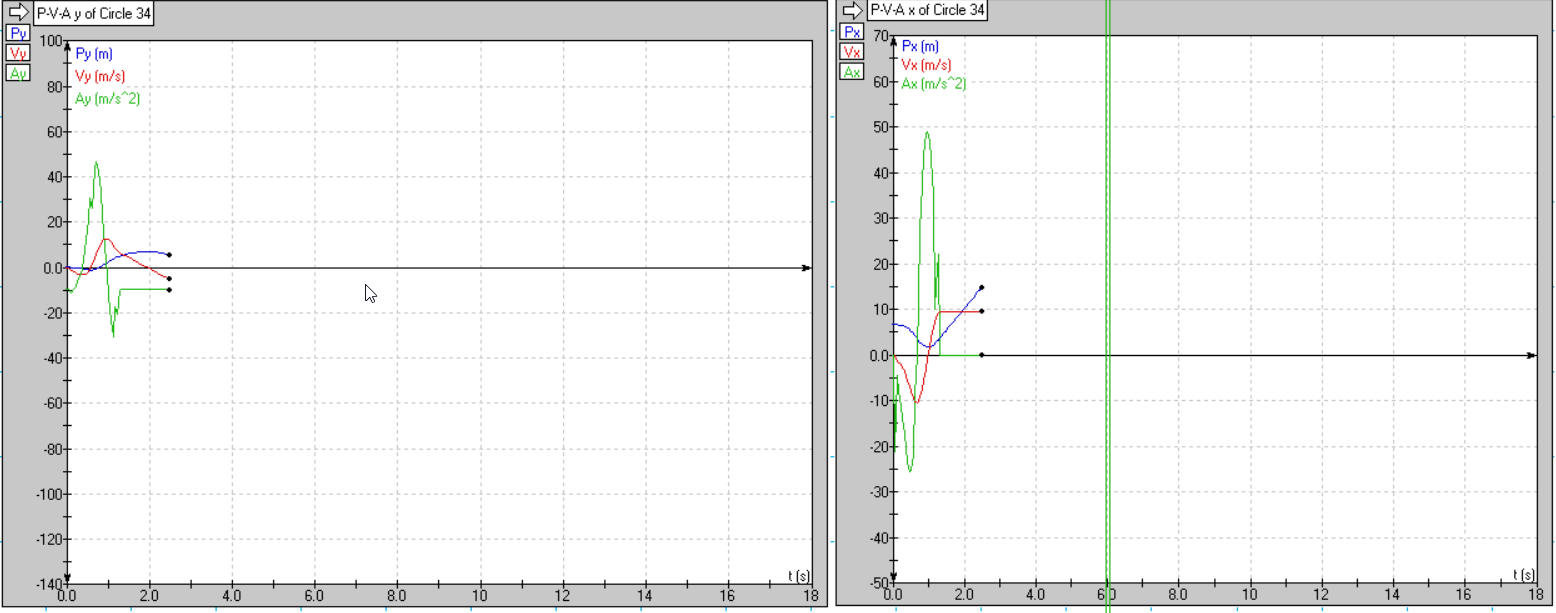
\includegraphics[width=\textwidth]{Graphs.png}
        \end{flushleft}
        \caption{P-V-A graph of ball\label{graphs}}
    \end{minipage}
    \hfill
    \begin{minipage}[t]{0.3\textwidth}
        \vspace{50pt}
        \begin{flushright}
            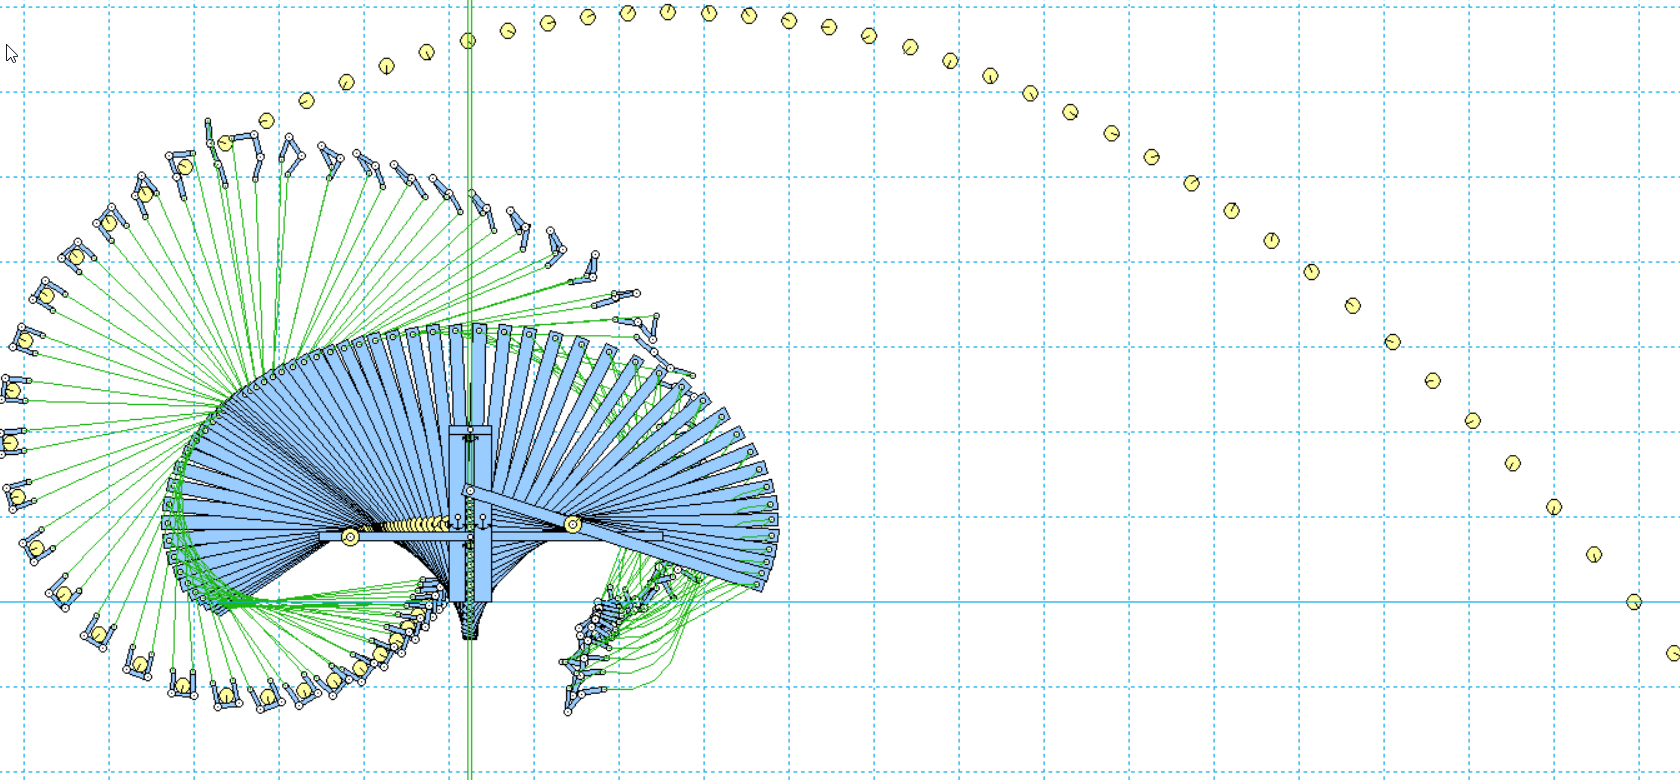
\includegraphics[width=\textwidth]{Motion.png}
        \end{flushright}
        \caption{Motion of Trebuchet\label{motion}}
    \end{minipage}
    \end{figure}
    \newpage
    \subsection{Real-life Data}

    \newpage
    \section{Comparison of Results}
    \newpage
    \section{Discussion}
    \newpage
    \section{Conclusions}
    The main objectives of this milestone were to create a blueprint for 
    the construction of the final build.
    The key findings are summarized as follows:
    \begin{enumerate}
        \item In order to maximize the distance traveled by the projectile, it is essential to optimize the projectile's velocity. 
        \item General plane motion increases projectile velocity by harnessing the speed of the falling counterweight.    
        \item Floating Arm Trebuchets consist of five main components: 
            frame, arm, counterweight, sling, and guide chute.
        \item The release of the projectile at a 45 degree angle achieves the 
            maximum projectile distance.
    \end{enumerate}
    \newpage
    \section{References}
        \hspace{15pt}Denny, M. (2005). Siege engine dynamics. European journal of physics, 26(4), 561.

        Hibbeler, R. C. (2015). 16.5. In Engineering mechanics: Dynamics (pp. 346–348). essay, Pearson.
        
        James O'Connell; Dynamics of a medieval missile launcher: the trebuchet. The Physics Teacher 1 November 2001; 39 (8): 471–473.

        Rhoten, R. P. (1999). The trebuchet: Accuracy analysis of a medieval siege engine. Volume 2: 19th Computers and Information in Engineering Conference.

        Siano, D. B. (2001). Trebuchet Mechanics. The Algorithmic Beauty of the Trebuchet.
\end{document}
